\documentclass[12pt]{article}
\usepackage{amsmath}
\usepackage{graphicx}
\usepackage{float}
\usepackage[utf8]{inputenc}
\usepackage{cite}
\usepackage{setspace}
\usepackage{amsfonts}
\usepackage{mathrsfs}
\usepackage[margin=1.0in]{geometry}
\usepackage{enumitem}
\usepackage{listings}

\numberwithin{equation}{section}

\title{Programming a Linear Algebra Solution to the Poisson Equation}
\author{Elizabeth Drueke}

\begin{document}
\maketitle

\begin{abstract}
Poisson's equation is vital in the study of the physical world.  In every subfield of physics, from mechanics and quantum mechanics to electromagnetism, we are able to model physical systems subject to boundary conditions with this versatile equation.  This means that developing computer programs which can quickly and accurately solve this equation is of the utmost importance.  Here, we develop a code using C++ compiled within the ROOT framework which can create a numerical approximation to the solution of the Poisson equation, specifically subject to the Dirichlet boundary conditions.  In the process, we also explore dynamic memory allocation in C++ and the use of classes.
\end{abstract}

\section{Introduction}
\label{sec:into}
It is important in physics to develop ways to deal with large quantities of data and to use that data to make close approximations of physical conditions.  In particular, we wish to develop computer programs which can both automate the process of numerical approximation and which can complete that approximation in a timely manner.  One example of an equation which we will often need to solve when investigating physical situations is the Poisson equation, given by 

\begin{equation}
\vspace{.2cm}
\label{eq:poisson}
-u''\left(x\right) = f\left(x\right),
\end{equation}

\noindent subject to the Dirichlet boundary conditions,

\begin{equation}
\vspace{.2cm}
\label{eq:dirichlet}
u\left(0\right)=u\left(1\right)=0.
\end{equation}

In this report, we will study various numerical approximations to solutions to the Poisson equation in great detail, particularly focusing on using linear algebra and the solutions of linear systems to determine a close approximation to the solution $u\left(x\right)$.  We pay special attention to the number of floating point operations (FLOPS) and the time required for various approximation methods.

\section{Theory}
\label{sec:theory}
The mathematics behind the solution to the Poisson equation presented here is mathematically rich in approximations.  From Eq.~\ref{eq:poisson}, we can see that we are required to compute the function $u\left(x\right)$ from its second derivative.  To do this, we note that we can always approximate the first derivative as

\begin{equation}
\vspace{.2cm}
\label{eq:deriv1}
f'\left(x\right) \approx \frac{f\left(x+h\right)-f\left(x-h\right)}{2h},
\end{equation}

\noindent for $h<<1$ because the derivative is the slope of the line tangent to $f$ at that point.  This then implies that

$$\begin{array}{ccc} f''\left(x\right)&\approx&\frac{f'\left(x+h\right)-f'\left(x-h\right)}{2h} \\
&\approx&\frac{\frac{f\left(x+h+h\right)-f\left(x+h-h\right)}{2h} - \frac{f\left(x-h+h\right)-f\left(x-h-h\right)}{2h}}{2h} \\
&\approx&\frac{\frac{f\left(x+2h\right)-f\left(x\right)}{2h} - \frac{f\left(x\right)-f\left(x-2h\right)}{2h}}{2h} \\
&\approx&\frac{f\left(x+2h\right)-2f\left(x\right)+f\left(x-2h\right)}{\left(2h\right)^{2}}.\end{array}$$

\noindent Letting $2h\rightarrow h$, we then have

\begin{equation}
\vspace{.2cm}
\label{eq:deriv2}
f''\left(x\right)\approx\frac{f\left(x+h\right)-2f\left(x\right)+f\left(x-h\right)}{h^{2}}.
\end{equation}

\noindent Eq.~\ref{eq:deriv2} will serve as our approximation to the second derivative throughout the remainder of this discussion.  
\\\indent Now, we have an expression which lends itself to the use of vectors.  Letting $$h = \frac{1}{n+1}$$ be the step size for some number of steps $n\in\mathbb{N}$, we see that we can treat this as a partition of the interval $\left[0,1\right]$, on which the Dirichlet conditions are valid.  Thus, we define each $x_{i}$ in the partition as $$x_{i}=ih,i=0,\ldots,n+1.$$  From these $x_{i}$ we can create a vector $\textbf{x}$\footnote{Note that throughout we indicate vectors as bold, lowercase letters (eg. $\textbf{x}$), and matrices as uppercase letters (eg. $A$).}

$$\textbf{x} = \left(0,\frac{1}{n+1},\frac{2}{n+1},\ldots,\frac{n}{n+1},1\right)^{T}.$$
\vspace{.2cm}

\noindent Then, let $\textbf{b}$ be a vector of the function $f\left(x\right)$ evaluated at the points in $\textbf{x}$.  That is,

$$\begin{array}{ccc}\textbf{b} &=& \left(f\left(0\right),f\left(\frac{1}{n+1}\right),f\left(\frac{2}{n+1}\right),\ldots,f\left(\frac{n}{n+1}\right),f\left(1\right)\right)^{T} \\ \vspace{.2cm}
&=& \left(0,f\left(\frac{1}{n+1}\right),f\left(\frac{2}{n+1}\right),\ldots,f\left(\frac{n}{n+1}\right),0\right)^{T}.
\end{array}$$
\vspace{.2cm}

\noindent Now, we see that Eq.~\ref{eq:deriv2} lends itself nicely to the introduction of a linear algebra problem.  In particular, we can define an $\left(n+1\right)\times \left(n+1\right)$ matrix $A$ such that

\vspace{.1cm}
\begin{equation}
\label{eq:a}
A = \frac{1}{h^{2}} \left(
\begin{array}{cccccc}
2 & -1 & 0 & \cdots & \cdots & 0 \\
-1 & 2 & -1 & 0 & \cdots & 0 \\
0 & -1 & 2 & -1 & 0 & \vdots \\
\vdots & \ddots & \ddots & \ddots & \ddots & \vdots \\
\vdots & \vdots & \vdots & \ddots & -1 & 2
\end{array}
\right)
\end{equation}
\vspace{.2cm}

\noindent Then, we have that the Poisson Equation given by Eq.~\ref{eq:poisson} can be approximated as 

\begin{equation}
\label{eq:avb}
A\textbf{v}=\textbf{b}
\end{equation}

\noindent for some $\textbf{v}$ which represents $u\left(x\right)$ at various values of $x$.  And so we have a system of $n+1$ equations in $n+1$ unknowns.  Once we have solved for the vector $\textbf{v}$, we can use a plotting tool to plot the points and extrapolate a fit to the function.
\\\indent In general, there are two main ways in which we might solve  Eq.~\ref{eq:avb}, known as Gaussian elimination and LU Decomposition.  We will discuss these in general in Section~\ref{subsec:gausselim} and Section~\ref{subsec:ludecomp}, respectively, before discussing how we developed the computer algorithms for these methods specifically for our matrix $A$ given by Eq.~\ref{eq:a} in Section~\ref{sec:algorithm}.

\subsection{Gaussian Elimination}
\label{subsec:gausselim}

Gaussian elimination is the method of solving linear systems typically taught in introductory linear algebra classes. This method involves adding multiples of rows of the matrix to other rows in order to eliminate (or set to zero) off-diagonal elements.  In order to determine a solution, any row operation performed on the matrix $A$ must be performed on our solution vector $\textbf{b}$\footnote{Following the notation in Eq.~\ref{eq:avb}.} in parallel.  In most situations, it is necessary to employ both a forward and backward Gaussian elimination method in order to solve a full system.  To demonstrate this method, we look at a $3\times 3$ example.  The algorithm used within the code will be more explicitly discussed in Section~\ref{sec:algorithm}.
\\\indent Suppose we have a matrix $A$ of the form

\begin{equation}
\label{eq:ainit}
A = \left(
\begin{array}{ccc}
a_{11} & a_{12} & a_{12} \\
a_{21} & a_{22} & a_{23} \\
a_{31} & a_{32} & a_{33}
\end{array}
\right)
\end{equation}
\vspace{.2cm}

\noindent and we wish to reduce it to row echelon form.  We might do this using Gaussian elimination.  To begin, we would use forward elimination to set the $a_{i1}$ components to zero for $i\neq1$.  Letting $R_{i}$ denote the $i^{th}$ row, we notice that letting 

\begin{equation}
\label{eq:rowops1}
\begin{align}
R_{2} & = R_{2} - \frac{a_{21}}{a_{11}}R_{1} \\
R_{3} & = R_{3} - \frac{a_{31}}{a_{11}}R_{1}
\end{align}
\end{equation}

\noindent should yield the desired outcome.  That is, we have 

\begin{equation}
\label{eq:gaussflops}
A = \left(
\begin{array}{ccc}
a_{11} & a_{12} & a_{13} \\
a_{21} & a_{22} & a_{23} \\
a_{31} & a_{32} & a_{33}
\end{array}
\right) \rightarrow \left(
\begin{array}{ccc}
a_{11} & a_{12} & a_{12} \\
0 & a_{22} - \frac{a_{21}a_{12}}{a_{11}} & a_{23} - \frac{a_{21}a_{13}}{a_{11}} \\
0 & a_{32} - \frac{a_{31}a_{12}}{a_{11}} & a_{33} - \frac{a_{31}a_{13}}{a_{11}}
\end{array}\right).
\end{equation}
\vspace{.2cm}

\noindent Continuing in this manner, we will eventually have a matrix of the form 

\begin{equation}
A\prime = \left(
\begin{array}{ccc}
a_{11}\prime & a_{12}\prime & a_{13}\prime \\
0 & a_{22}\prime & a_{23}\prime \\
0 & 0 & a_{33}\prime
\end{array}\right),
\end{equation}
\vspace{.2cm}

\noindent where the $\prime$ indicates that the element has been modified from its original definition in Eq.~\ref{eq:ainit}.  
\\\indent At this point, we may begin the backward Gaussian elimination process.  In the forward process, we were able to set all of the $a_{ij}=0$ for $i>j$.  In the backward process, we wish to do the same for the $a_{ij}$ with $i<j$.  In the end, we should have a pure diagonal matrix.
\\\indent To begin the backward process, we note that we can set the $a_{i3}$ elements to zero by similar calculations as those performed in Eq.~\ref{eq:rowops1}.  In particular, we can let 

\begin{equation}
\label{eq:rowops2}
\begin{align}
R_{2} &= R_{2} - \frac{a_{23}}{a_{33}}R_{3} \\
R_{1} &= R_{1} - \frac{a_{13}}{a_{33}}R_{3}
\end{align}
\end{equation}

\noindent Doing this, we see 

$$\left(
\begin{array}{ccc}
a_{11}\prime & a_{12}\prime & a_{13}\prime \\
0 & a_{22}\prime & a_{23}\prime \\
0 & 0 & a_{33}\prime
\end{array}\right) \rightarrow
\left(\begin{array}{ccc}
a_{11}\prime & a_{12}\prime & 0 \\
0 & a_{22}\prime & 0 \\
0 & 0 & a_{33}\prime 
\end{array}\right).$$
\vspace{.2cm}

\noindent Continuing in this manner, we can see that we will eventually come across a pure diagonal matrix.  From here, having performed the row operations on the solution vector $\textbf{b}$ as well as the matrix $A$, we can find our solution $\textbf{v}$ by noting that 

\begin{equation}
v_{i} = \frac{\widetilde{b_{i}}}{\widetilde{a_{ii}}},
\end{equation}
\vspace{.1cm}

\noindent where the $\sim$ indicates that this is the component of the fully Gaussian eliminated matrix/vector.  This procedure is easily generalized to work for any $n\times n$ matrix.
\\\indent One downside to this method of solving the system of linear equations is that whatever row operations are performed on $A$ in Eq.~\ref{eq:avb} must also be performed on $\textbf{b}$.  This means that the process must be repeated every time the solution vector is changed.  This restriction can be a serious time constraint on any program written to implement Gaussian elimination in order to solve systems of linear equations.  The time limitations of such an algorithm are discussed in Section~\ref{sec:algorithm}.

\subsection{LU Decomposition}
\label{subsec:ludecomp}

The second major linear system solving method is what is known as LU decomposition.  In this procedure, we decompose our $A$ matrix into a lower-triangular $L$ and an upper-triangular $U$ of the form

\begin{equation}
\label{eq:ludecomp1}
\begin{array}{cccc}
\left(
\begin{array}{ccc}
a_{11} & a_{12} & a_{13} \\
a_{21} & a_{22} & a_{23} \\
a_{31} & a_{32} & a_{33}
\end{array}
\right) &=&
\left(
\begin{array}{ccc}
1 & 0 & 0 \\
l_{21} & 1 & 0 \\
l_{31} & l_{32} & 1
\end{array}\right)&
\left(\begin{array}{ccc}
u_{11} & u_{12} & u_{13} \\
0 & u_{22} & u_{23} \\
0 & 0 & u_{33}
\end{array}\right) \\
A &=& L&U
\end{array}
\end{equation}

\noindent In contrast with the Gaussian elimination method, this method does not need to be repeated for every choice of solution vector $\textbf{b}$.  Instead, once $L$ and $U$ have been computed, they can be used to determine the solution $\textbf{v}$ for any solution vector $\textbf{b}$.
\\\indent As with the Gaussian elimination method, we present an example as an illustration of how the LU decomposition method works.  Assume we have some 

\begin{equation}
\label{eq:ainit2}
A = \left(\begin{array}{cccc}
a_{11} & a_{12} & a_{13} & a_{14} \\
a_{21} & a_{22} & a_{23} & a_{24} \\
a_{31} & a_{32} & a_{33} & a_{34} \\
a_{41} & a_{42} & a_{43} & a_{44}
\end{array}\right).
\end{equation}
\vspace{.2cm}

\noindent Based on the multiplication as shown in Eq.~\ref{eq:ludecomp1}, we can see that we can directly solve for the $l_{ij}$ and $u_{ij}$.  In particular, in order, we see\footnote{Here, the boldface text indicates the unknown variable in each equation.}

\begin{equation}
\begin{align}
a_{11} =& {\bf u_{11}} &\Rightarrow \\
a_{21} =& {\bf l_{21}} u_{11} &\Rightarrow \\
a_{31} =& {\bf l_{31}}u_{11} &\Rightarrow \\
a_{41} =& {\bf l_{41}}u_{11} &\Rightarrow \\
a_{12} =& {\bf u_{12}} &\Rightarrow \\
a_{22} =& {\bf l_{21}}u_{12}+u_{22} &\Rightarrow \\
a_{32} =& l_{31}u_{12}+{\bf l_{32}}u_{22} &\Rightarrow \\
a_{42} =& l_{41}u_{12}+{\bf l_{42}}u_{22} &\Rightarrow \\
a_{13} =& {\bf u_{13}} &\Rightarrow \\
a_{23} =& l_{21}u_{13}+{\bf u_{23}} &\Rightarrow \\
a_{33} =& l_{31}u_{13}+l_{32}u_{23}+{\bf u_{33}} &\Rightarrow \\
a_{43} =& l_{42}u_{23}+{\bf l_{43}}u_{33}+l_{41}u_{13} &\Rightarrow \\
a_{14} =& {\bf u_{14}} &\Rightarrow \\
a_{24} =& l_{21}u_{14}+{\bf u_{24}} &\Rightarrow \\
a_{34} =& l_{31}u_{14}+l_{32}u_{24}+{\bf u_{34}} &\Rightarrow \\
a_{44} =& l_{41}u_{14}+l_{42}u_{24}+l_{43}u_{34}+{\bf u_{44}}. &
\end{align}
\end{equation}
\vspace{.2cm}

\noindent This result generalizes to any $n\times n$ matrix.  In particular, an algorithm can be developed which will always give the $L$ and $U$ matrix from known values.  This algorithm, known as Doolittle's Algorithm[2], proceeds as follows:

\begin{itemize}
\item Starting with column $j=1$, compute the first element by 

\begin{equation}
\label{eq:ludecomp1}
u_{1j}=a_{1j}
\end{equation}

\item For $i=2,\ldots,j-1$, compute

\begin{equation}
\label{eq:ludecomp2}
u_{ij}=a_{ij}-\sum_{k=1}^{i-1}l_{ik}u_{kj}
\end{equation}

\item Calculate the diagonal element as

\begin{equation}
\label{eq:ludecomp3}
u_{jj}=a_{jj}-\sum_{k-1}^{j-1} l_{jk}u_{kj}
\end{equation}

\item Calculate the $l_{ij}$ for $i>j$ as

\begin{equation}
\label{eq:ludecomp4}
l_{ij}=\frac{1}{u_{jj}}\left(a_{ij}-\sum_{k=1}^{j-1} l_{jk}u_{kj}\right)
\end{equation}

\item Repeat with columns $j=2,3,\ldots,n$.
\end{itemize}

\noindent Of course, this algorithm does not actually compute the solution to the linear system presented in Eq.~\ref{eq:avb}.  To compute the solution $\textbf{v}$, we must invoke another algorithm.  To begin, we note that

\begin{equation}
\label{eq:axbluxb}
A\textbf{v}=\textbf{b}\Rightarrow LU\textbf{v}=\textbf{b}.
\end{equation}
\vspace{.05cm}

\noindent This implies that we should be able to define an intermediate vector $\textbf{y}=U\textbf{v}$ which can be easily computed.  In the four-dimensional example, we would have the set of equations

$$\begin{array}{rcc} u_{44}v_{4}&=&y_{4} \\
u_{33}v_{3}+u_{34}v_{4}&=&y_{3} \\
u_{22}v_{2}+u_{23}v_{3}+u_{24}v_{4}&=&y_{2} \\
u_{11}v_{1}+u_{12}v_{2}+u_{13}v_{3}+u_{14}v_{4}&=& y_{1} \end{array}$$

\noindent and

$$\begin{array}{rcc}y_{1}&=&b_{1} \\
l_{21}y_{1}+y_{2}&=&b_{2} \\
l_{31}y_{1}+l_{32}y_{2}+y_{3}&=&b_{3} \\
l_{41}y_{1}+l_{42}y_{2}+l_{43}y_{3}+y_{4}&=&b_{4}.\end{array}$$
\vspace{.2cm}

\noindent Thus, there must be both an algorithm to decompose the matrix $A$ into an upper-triangular $U$ and a lower-triangular $L$ and another algorithm to actually compute the solution to Eq.~\ref{eq:avb} from that $L$ and $U$.
\\\indent One benefit to using LU decomposition over Gaussian elimination, aside from the fact that it will take less time than the standard Gaussian elimination method,\footnote{The specific argument to this statement is presented in Section~\ref{subsec:timedependence}.}  is that it is very natural to compute the determinant of the matrix once it has been LU-decomposed.  This is because we have 

$$A=LU \Rightarrow \det\left(A\right)=\det\left(LU\right)=\det\left(L\right)\det\left(U\right),$$

\noindent and the determinant of either an upper-triangular or lower-triangular matrix is simply the product of its diagonal elements.  Because $L$ has 1's along its diagonal, we can see that

\begin{equation}
\det\left(A\right)=\prod_{i=1}^{n}u_{ii}.
\end{equation}
\vspace{.2cm}

\section{The Algorithm}
\label{sec:algorithm}

The meat of this project is the development of an algorithm which can compute a fair approximation for $u\left(x\right)$ in Eq.~\ref{eq:poisson}.  In order to check our solutions, we take our function $f$ to be given by $f\left(x\right) = 100e^{-10x}$.  We work with the linear algebra solutions described in Section~\ref{sec:theory}.  The code written to this end is written using C++ and is compiled using ROOT v5.34/12[1].  All plots are made within the program using ROOT plotting features.
\\\indent Within the code, it is first necessary to define our matrix $A$ as in Eq.~\ref{eq:a} and a vector of solutions $\textbf{b}$ as in Eq.~\ref{eq:avb}.  Noting that, in fact, we know the solution for $u\left(x\right)$ at $x=0$ and $x=1$\footnote{These values are given by the Dirichlet boundary conditions.}, we do not include either the $x_{0}$ or $x_{n+1}$\footnote{In the notation of $x_{i}=ih,i=0,\ldots,n+1$ where $h=\frac{1}{n+1}$.} terms.  However, when we perform the fit to our plot at the end, these boundary conditions will be included for completeness.  To declare these objects, we create classes $\texttt{themat}$ and $\texttt{thevec}$ for matrices and vectors handled with dynamic memory. 
\\\indent The classes and function definitions come in documents $\texttt{classes.h}$ and $\texttt{classes.C}$.  Every object of the $\texttt{thevec}$ class has associated with it an integer $\texttt{sz}$ which is the number of rows of the vector, and a pointer to a dynamic memory array $\texttt{point}$ in which we can place the values of the components of the vector.  This class comes equipped with several constructors, a destructor (which de-allocates any memory in use by the object), several overloaded operators (addition of two vectors, subtraction of two vectors, multiplication of two vectors (in the form of a dot product), etc.), a component retrieval function ($\texttt{operator[]}$) which returns the value of the vector at a particular index, and a printing member function.  
\\\indent The setup of the $\texttt{themat}$ class is very similar to that of the $\texttt{thevec}$ class.  The $\texttt{sz}$ component here is the $n$ which defines the matrix (ie. creates an $n\times n$ matrix) and the $\texttt{point}$ is a double pointer.  This class also comes with multiple constructors, several overloaded operators (including matrix-matrix and matrix-vector multiplication), a component-retrieval function, and a print function.  For ease of use, $\texttt{thevec}$ was declared as a friend function of $\texttt{themat}$.  
\\\indent Once the vector and matrix objects are defined, it is just a matter of solving Eq.~\ref{eq:avb} using the matrix and vector specific to the problem.  However, because we are working with a specific kind of matrix, there are several things we can do to reduce the computing power needed to solve the problem.  The first is noting that we do not have to proceed with the full LU-decomposition in order to decompose our special matrix.  Looking at a $4\times4$ example, we see a pattern forming. 

\begin{equation}
\begin{array}{cccc}
\left(\begin{array}{cccc}
1 & 0 & 0 & 0 \\
-\frac{1}{2} & 1 & 0 & 0 \\
0 & -\frac{2}{3} & 1 & 0 \\
0 & 0 & -\frac{3}{4} & 1 
\end{array}\right) &
\left(\begin{array}{cccc}
2 & -1 & 0 & 0 \\
0 & \frac{3}{2} & -1 & 0 \\
0 & 0 & \frac{4}{3} & -1 \\
0 & 0 & 0 & \frac{5}{4} 
\end{array}\right) &=&
\left(\begin{array}{cccc}
2 & -1 & 0 & 0 \\
-1 & 2 & -1 & 0 \\
0 & -1 & 2 & -1 \\
0 & 0 & -1 & 2
\end{array}\right) \\
L & U & = & A.
\end{array}
\end{equation}

\noindent In general, then, we might suppose that the matrix elements $l_{ij}$ and $u_{ij}$ of $L$ and $U$ will take the form

\begin{equation}
\label{eq:luspecalg}
\begin{array}{cc}
l_{ii} = 1, & l_{i,i-1} = -\frac{i-1}{i-2}, \\
u_{ii} = \frac{i+1}{i}, & u_{i,i+1}=-1
\end{array}
\end{equation}
\vspace{.2cm}

\noindent and all other $l_{ij}$ and $u_{ij}$ are 0.  Noticing this means that we are required to perform far fewer float operations in order to decompose the matrix.  
\\\indent From there, it becomes simpler to solve the linear system as well.  Referring back to the $4\times4$ example, we can now solve for our intermediate $\textbf{y}$ and then our solution $\textbf{v}$ with the following equations:

\begin{equation}
\label{eq:easylusolver}
\begin{array}{ccc}
\begin{array}{c}
y_{1}=b_{1} \\
-\frac{1}{2}y_{1}+y_{2}=b_{2} \\
-\frac{2}{3}y_{2}+y_{3}=b_{3} \\
-\frac{3}{4}y_{3}+y_{4}=b_{4} \\
-\frac{4}{5}y_{4}+y_{5}=b_{5}
\end{array} & \rightarrow &
\begin{array}{c}
2v_{1}-v_{2}=y_{1} \\
\frac{3}{2}v_{2}-v_{3}=y_{2} \\
\frac{4}{3}v_{3}-v_{4}=y_{3} \\
\frac{5}{4}v_{4}-v_{5}=y_{4} \\
\frac{6}{5}v_{5}=y_{5}
\end{array}
\end{array}
\end{equation}
\vspace{.2cm}

\noindent In fact, with the matrix as specific as it is, it isn't necessary even to pass the $L$ and $U$ matrices to the solving algorithm in order to solve the system.  Instead, one possible version of the algorithm is:

\vspace{.4cm}
\begin{1stlisting}
\texttt{y[0]=b[0]; \\ \indent for(int i=1;i<n;i++)\{ \\ \indent\indent y[i]=b[i]+(i/(i+1))*y[i-1]; \\\indent \} \\\indent v[n-1] = n*y[n-1]/(n+1); \\ \indent
for(int i=n-2;i>-1;i--)\{ \\\indent \indent v[i]=((i+1)/(i+2))*(y[i]+v[i+1]); \\\indent \}}
\end{1stlisting}
\vspace{.4cm}

\noindent However, the main goal of rewriting the algorithm specific to the matrix required to solve the Poisson equation is to reduce the number of FLOPs, and writing the program in this way will actually force the computer to perform unnecessary floating point operations because the fractional factors will have already been computed in the LU decomposition step.  It is for this reason that we create an essentially shorter version of the LU decomposition solving function, which works with the already-computed elements of the $L$ and $U$ matrices.  In particular, our algorithm first solves for the intermediate vector $\textbf{y}$ as 

\vspace{.4cm}
\begin{1stlisting}
\texttt{y[0]=b[0]; \\\indent for(int i=0;i<n;i++)\{ \\\indent\indent y[i]=b[i]-L[i][i-1]*y[i-1]; \\\indent\}}
\end{1stlisting}
\vspace{.4cm}

\noindent and then solves for the solution to the problem $\textbf{v}$ as

\vspace{.4cm}
\begin{1stlisting}
\texttt{v[n-1]=y[n-1]/U[n-1][n-1]; \\\indent for(int i=n-2;i>-1;i--)\{ \\\indent\indent v[i]=(y[i]+v[i+1])/U[i][i];\\\indent\}}
\end{1stlisting}
\vspace{.4cm}

\noindent In this way, we are able to reasonably minimize the number of FLOPs required for the calculation.  A full analysis of the expected and observed time dependences of these algorithms is presented in Section~\ref{subsec:timedependence} and Section~\ref{sec:results}.
\\\indent In the end, our algorithm was fairly straightforward.  The full code to run the algorithm, complete with time and error analysis and a full solution for our particular test function, is contained in $\texttt{project1.C}$.  The brunt of the coding in this document involves the graphing utilities required to output the graphs in this paper, but the general layout of the code here is as follows:

\begin{itemize}
\item Determine the difference in the timing between the various linear solving algorithms using functions $\texttt{check\_timing\_all()}$ and $\texttt{check\_timing\_short()}$, which are included in this file.
\item Compute the errors and store them in $\texttt{plots/errors.txt}$.
\item Create a vector of the various numbers of steps we wish to compute a solution for and loop through it, calculating the solution within the function $\texttt{make\_sol\_plots\_()}$, which is within this file and calls the special LU decomposition solvers, $\texttt{LU\_decomp\_special()}$ and $\texttt{LU\_decomp\_solver\_special()}$, which are declared in $\texttt{classes.h}$ and defined in $\texttt{classes.C}$.  
\item Create the solution plots in directory $\texttt{plots/}$.
\end{itemize}

\\\indent Our final special LU decomposition solver is, as mentioned above, implemented in two different functions, $\texttt{LU\_decomp\_special()}$ and $\texttt{LU\_decomp\_solver\_special()}$, which are declared in $\texttt{classes.h}$ and defined in $\texttt{classes.C}$.  The algorithm in for these functions is as follows:

\begin{itemize}
\item For $\texttt{LU\_decomp\_special()}$:
\end{itemize}
\\\indent\indent\indent\texttt{for(int i=0;i<n;i++)\{ }
\\\indent\indent \indent \texttt{for(int j=0;j<n;j++)\{}
\\\indent\indent \indent \indent \texttt{if(i==j)\{}
\\ \indent\indent\indent\indent\indent \texttt{U[i][j]=(i+2)/(i+1);}
\\\indent\indent \indent\indent\indent \texttt{L[i][j]=1;}
\\\indent\indent \indent\indent \texttt{\}} 
\\\indent\indent \indent\indent \texttt{else if((i-1==j)\{} 
\\\indent\indent\indent\indent\indent \texttt{L[i][j]=-j/i;} 
\\\indent\indent \indent\indent\indent \texttt{U[i][j]=0;} 
\\ \indent\indent\indent\indent\textt{\}}
\\\indent\indent\indent\indent \texttt{else if(i+1==j)\{}
\\\indent\indent\indent\indent\indent \texttt{L[i][j]=0;}
\\\indent\indent\indent\indent\indent \texttt{U[i][j]=0;} 
\\\indent\indent\indent\indent\textt{\}}
\\\indent\indent\indent\indent \texttt{else\{}
\\\indent\indent\indent\indent\indent \texttt{L[i][j]=0;} 
\\\indent\indent\indent\indent\indent \texttt{U[i][j]=0;}
\\\indent\indent\indent\indent\texttt{\}}
\\\indent\indent\indent\textt{\}}
\\\indent\indent\texttt{\}}
\\\indent\indent\texttt{for(int i=0;i<n;i++)\{}
\\\indent\indent\indent \texttt{if(i!=(n-1))}
\\\indent\indent\indent\indent \texttt{L[i][i-1]=L[i+1][i];}
\\\indent\indent\indent \texttt{else} 
\\\indent\indent\indent\indent \texttt{L[i][i-1] = -1/(i+1);}
\\\indent\indent\texttt{\}}
\begin{itemize}
\item For $\texttt{LU\_decomp\_solver\_special()}$:
\end{itemize}
\\\indent\indent\indent\texttt{y[0]=b[0];}
\\\indent\indent\texttt{for(int i=0;i<n;i++)\{}
\\\indent\indent\indent\texttt{y[i]=b[i]-L[i][i-1]*y[i-1];}
\\\indent\indent\texttt{\}}
\\\indent\indent\texttt{v[n-1]=y[n-1]/U[n-1][n-1];}
\\\indent\indent\texttt{for(int i=n-2;i>-2;i--)\{}
\\\indent\indent\indent\texttt{v[i]=(y[i]+v[i+1])/U[i][i];}
\\\indent\indent\texttt{\}}
\vspace{.4cm}

\\\indent The algorithms written for the full Gaussian elimination and LU decomposition are based on the information in Sections~\ref{subsec:gausselim} and~\ref{subsec:ludecomp}.  Their composition is unenlightening and will not be explained in full detail here, although the code itself is well commented.

\subsection{Time Dependence}
\label{subsec:timedependence}

As mentioned in Section~\ref{sec:algorithm}, we wish to develop an algorithm which is not only able to solve numerically the Poisson equation, but which can also do so within a reasonable time frame and with limited computer memory usage. The amount of time required to run the algorithm is directly related to the number of FLOPs within that algorithm.  Here, we claim, based on counting the FLOPs in each argument, that the Gaussian elimination method will be the slowest of the three algorithms, while the special LU decomposition algorithm will be the quickest.
\\\indent Looking at the Gaussian elimination method, particularly at Eq.~\ref{eq:gaussflops}, we see that, for every step in the elimination process of the matrix, for every row we will have to compute a factor (eg. $\frac{a_{21}}{a_{11}}$ or $\frac{a_{31}}{a_{11}}$ as shown in Eq.~\ref{eq:gaussflops}), which will give us $n-1$ factors, and then one multiplication and one subtraction per element which will be $2\left(n-1\right)\left(n-1\right)$ FLOPs.  For the elimination process performed on the solution vector, we see that we will already have the factor required computed from the matrix step, and so we will only need to perform a subtraction and multiplication for each row of the solution vector, which yields $2\left(n-1\right)$ FLOPs.  Thus, to highest order, we expect the number of operations to go as $2\sum_{i=1}^{n-1}\left(n-i\right)\left(n-i\right)$.  Letting $j=n-i$, we see that we have the number of FLOPs going as 

$$2\sum_{i=1}^{n-1}j^{2} = \frac{2}{3}n\left(n+1\right)\left(2n+1\right),$$

\noindent and so we expect the leading term of the number of FLOPs to go as $\sim\frac{2}{3}n^{3}$.  Secondary terms go as $\sim n^{2}$ so we can consider them negligible.
\\\indent For the case of LU decomposition, we must look separately at the number of FLOPs required to decompose the matrix into an upper-triangular $U$ and a lower-tirangular $L$, and at the algorithm required to compute the solution vector from those decomposed matrices.  For the decomposition process, as shown in Eq.~\ref{eq:ludecomp1}-~\ref{eq:ludecomp4}, we see immediately that we get the $u_{1j}$ components for free from the original matrix.  Then for each column $j$, we have $j-2$ multiplication and subtraction steps to determine the $u_{ij}$ for a total of $2\left(j-2\right)\left(j-1\right)$.  Then, to compute the $u_{jj}$ components we have to multiply and subtract an additional $j-1$ times, and so our total becomes $2\left(j-1\right)\left(j-1\right)$.  Finally, for the $l_{ij}$ computations, we have $j-1$ multiplication and subtraction operations, and then one final division.  For every full column loop in our algorithm then, we should have $2j\left(j-1\right)$ FLOPs.  For $n$ columns, then, we should have 

$$2\sum_{j=1}^{n}j\left(j-1\right) = \frac{2}{3}n\left(n^{2}-1\right)$$

\noindent[3], which is the same as the dependence for Gaussian elimination.  However, for the actual solver, we have that there are $\sum_{i=1}^{n}2i$ FLOPs required to determine the intermediate vector $\textbf{y}$ and the same number to determine the solution vector from that intermediate vector.  So the total number of flops required to solve any system after the initial $\sim\frac{2}{3}n^{3}$ dependence is only 

$$2\sum_{i=1}^{n}2i = 2n\left(n+1\right)$$

\noindent[3] which goes as $\sim2n^{2}$.  From this, we can see that, particularly for problems involving multiple linear systems, LU decomposition will be faster than Gaussian elimination, which will go as $\sim n^{3}$ for all iterations.
\\\indent With our special matrix, however, we can cut this dependence down even further.  In particular, to complete the decomposition as in Eq.~\ref{eq:luspecalg}, we see that we will only need $n-1$ FLOPs for the $L$ matrix and $n$ flops for the $U$ matrix.  So the full decomposition will have a mere $2n-1$ flops.  The special solver, as we've defined it, will only require $n-1$ multiplication and subtraction steps each to determine the intermediate vector, and an additional $n-1$ multiplication and subtraction steps for the final solution calculation.  This means that, overall, our special LU decomposition and solver combined will require only $2n-1+4\left(n-1\right) = 6n-5$ FLOPs, which is significantly fewer than either the full LU decomposition or the full Gaussian elimination methods.  It is for this reason that, in our final code, the special LU decomposition algorithm was used for the calculations.

\section{Results and Benchmarks}
\label{sec:results}

Before entering a discussion of the full results of the program developed, it is important to validate the code appears to function properly.  In particular, it is reasonable to assume that, if all three algorithms written predict the same solution vector, then the solution is correct.  Such an analysis is performed in the $\texttt{benchmarks.C}$ file.  In this file, a matrix of the special form is created with varying dimensions between $1\times1$ and $50\times50$ and the resulting solution vector $\textbf{v}$ is computed using the full Gaussian elimination method ($\texttt{gauss\_elim()}$), the full LU decomposition solver ($\texttt{LU\_decomp()}$ together with $\texttt{LU\_decomp\_solver()}$), and the special LU decomposition solver which will work only on matrices of our specific form ($\texttt{LU\_decomp\_special()}$ together with $\texttt{LU\_decomp\_solver\_special()}$).  The results of these tests are found in $\texttt{benchmarks.txt}$.  It is shown here that, for a specific $A$, all three algorithms return precisely the same solution vector $\textbf{v}$.  In addition, the $L$ and $U$ matrices created by the different LU Decomposition algorithms are also identical and, when multiplied together, yield our original matrix $A$.
\\\indent We now discuss the results of the analysis.  Because of the simplicity of our test function, $f\left(x\right)=100e^{-10x}$, we can directly compute $u\left(x\right)$ either by hand or with any computing software.  We chose to use WolframAlpha [3].  We find that, subject to the Dirichlet boundary conditions, the solution is given by 

\begin{equation}
\label{eq:expectsol}
u\left(x\right)=\frac{x}{e^{10}}-x-e^{-10x}+1
\end{equation}

\\\indent The results for various numbers of steps are plotted in Figure~\ref{fig:result}.  From the image, it appears that increasing the number of steps greatly improves the validity of the result.  In fact, by the $n=51$ case, the calculated solution appears to follow the expected solution almost exactly.  In particular, we can determine how close our approximation is by computing the relative error $\epsilon_{i}$ between the expected value $u_{exp}$ of the function at point $x_{i}$ and the result computed by our special LU decomposition algorithm $u_{comp}$ as 

\begin{equation}
\label{eq:relerror}
\epsilon_{i} = \log_{10}\left(\left|\frac{u_{comp}-u_{exp}}{u_{exp}}\right|\right).
\end{equation}

\noindent The maximum value of $\epsilon_{i}$ for a collection of step values for each of the three solvers investigated is listed in Table~\ref{tab:errors}.  This confirms our suspicions that the error decreases with increasing number of steps.  Because the errors are the same for each algorithm, we have yet another confirmation (aside from the benchmark) that our algorithm is working correctly.  In particular, we might expect that, at much higher numbers of steps, the error would again start to increase.  This is because the numbers in the algebra would cease to be within the range of type $\texttt{double}$.  As it is, however, we do not yet observe this behavior.

\begin{figure}[h]
\label{fig:result}
\begin{center}
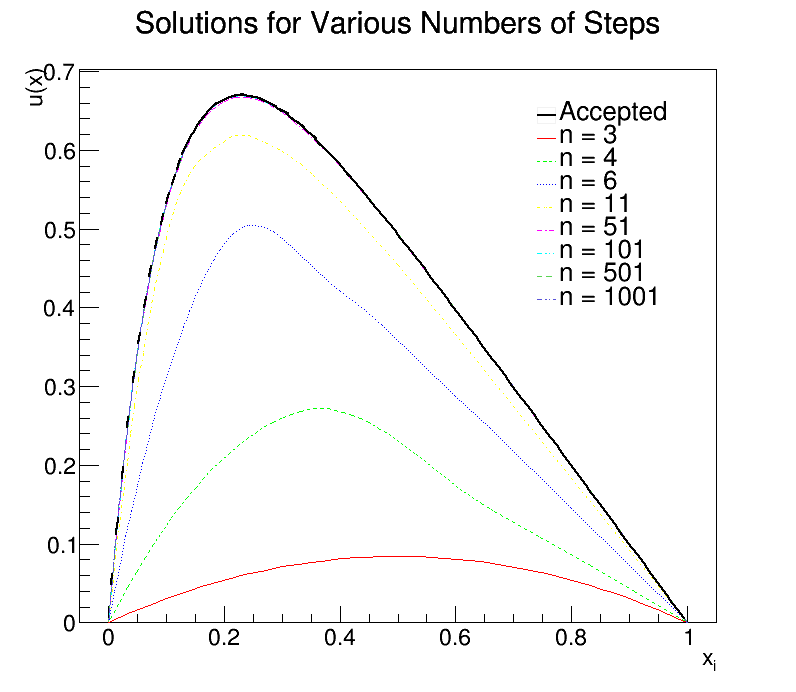
\includegraphics[width=0.55\textwidth]{plots/solution_plot}
\caption{The results of the special LU decomposition algorithm plotted with the accepted solution (Eq.~\ref{eq:expectsol}).}
\end{center}
\end{figure}

\begin{table}[!h!tbp]
\label{tab:errors}
\begin{center}
\begin{tabular}{c|c|c|c}
\hline
Number of Steps & Gaussian Elimination & Full LU Decomp. & Special LU Decomp. \\
\hline
4 & -0.559188 &-0.559188  & -0.559188 \\
10 & -1.1797 & -1.1797& -1.1797 \\
50 & -2.49516 & -2.49516 & -2.49516 \\
100 & -3.08804 & -3.08804 & -3.08804 \\
500 & & & -4.47887 \\
1000 & & & -5.08005 \\
10000 & & & -7.07927 \\
\hline
\end{tabular}
\caption{The maximum errors as computed in Eq.~\ref{eq:relerror} by the number of steps for each of the three linear system solvers investigated..}
\end{center}
\end{table}

\\\indent We were also able to perform a cursory analysis of the real-time differences between the various algorithms.  The results of this analysis are shown in Figures~\ref{subfig:a} and~\ref{subfig:b}.  From these figures, we can see that our initial hypotheses were correct and the special LU decomposition solver's step dependence is far lower than those of the full LU decomposition and the full Gaussian decomposition.

\begin{figure}[h]
\begin{center}
\begin{subfigure}
\label{subfig:a}
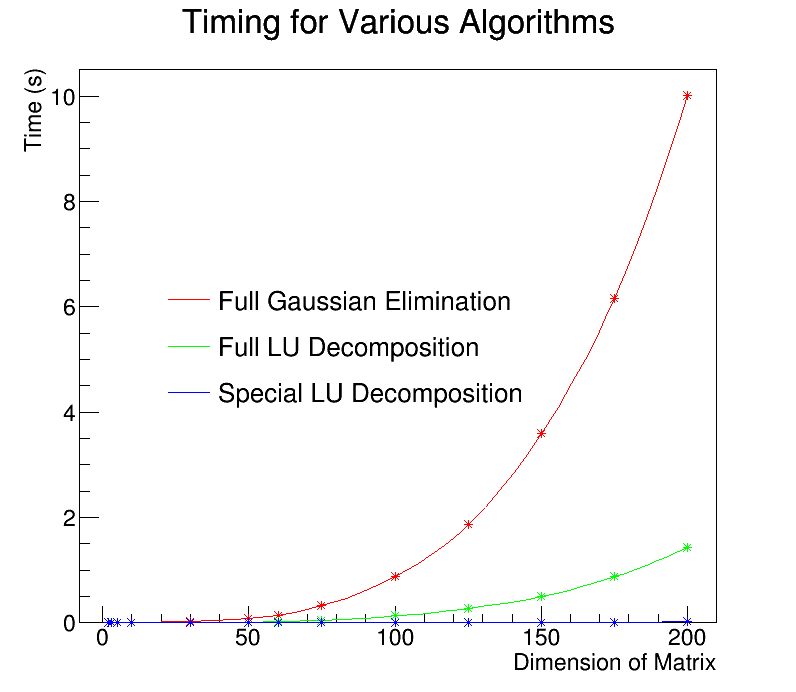
\includegraphics[width=0.45\textwidth]{plots/time_plot}
\end{subfigure}
\begin{subfigure}
\label{subfig:b}
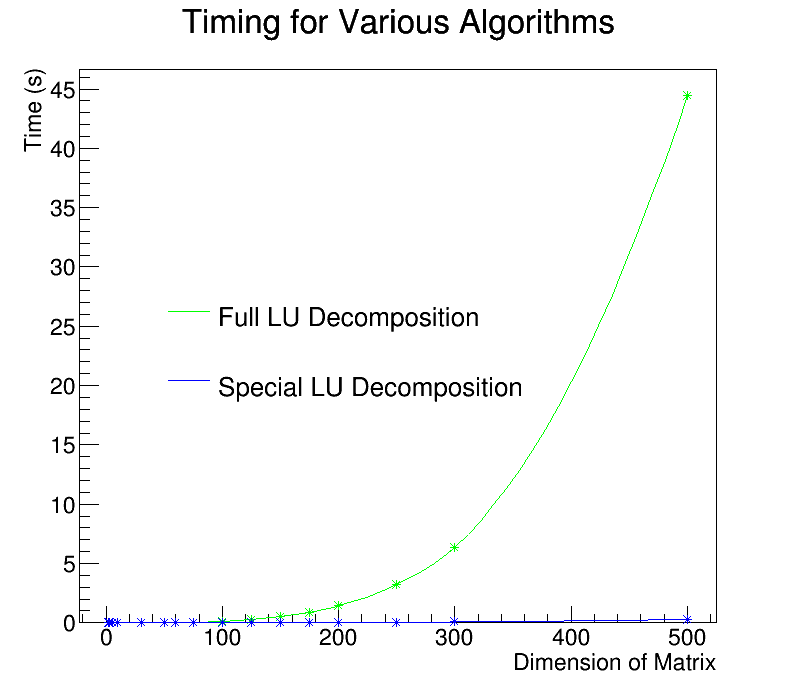
\includegraphics[width=0.45\textwidth]{plots/time_plot_short}
\end{subfigure}
\caption{The observed dependences of the various algorithms on the dimension of the matrix used  Here, we see that the full Gaussian algorithm takes far longer than either LU decomposition algorithm, and that our special LU decomposition really does cut down the time from the full LU decomposition algorithm.  This observations serves as a justification for why we chose to use the lesser-known algorithm we do know.  The plot on the left shows all three algorithms while the plot on the right shows both LU decomposition algorithms and emphasizes their differences at larger dimension sizes.}
\end{center}
\end{figure}

\section{Conclusions}
\label{sec:conclusions}

In all, our Poisson equation solver appears to run with reasonable efficiency and accuracy.  We can see from Table~\ref{tab:errors} that the relative error of the numerical approximation by our special LU decomposition solver decreases with decreasing step size.  This is expected because, if we think about the limit definition of the derivative (as mentioned in Eq.~\ref{eq:deriv1}), the derivative is taken as $h\rightarrow0$.  By increasing the number of steps, we are decreasing the step size ($h$-value) and are therefore more closely approximating the derivative.  We were also able to confirm that our special LU decomposition solver was faster than the full LU decomposition solver or the full Gaussian elimination solver, which were both developed for this project.  
\\\indent These successes do not, however, imply that the program developed for the solution to this Poisson equation problem is perfect.  One major issue was the time required by even the special LU decomposition solver to compute a $10000\times10000$ matrix.  Our goal for this project was to develop a code which could run with the highest efficiency, which suggests more time should be spent trying to perfect the algorithm and further limit its FLOP dependence.  Although it took an average of over half an hour to run the code in full, however, it is important to note that the computer on which the code was run for this analysis is used by multiple people for large, computing-intensive physics jobs.  It is very possible that someone was computing on the computer at the same time this analysis was being run, thus slowing it down.  However, that information is not presently available.
\\\indent It should also be noted that the classes developed within the context of this project do leave much to be desired.  They have not been fully tested outside of being able to handle our special matrix in a non-special way.  This means, for example, that given a matrix with a 0 on the diagonal, our full Gaussian elimination algorithm may find itself dividing by 0.  There are also several functions, like the $\texttt{print()}$ function in both classes, which could afford some edits in order to perfect them.  In the case of $\texttt{print()}$ it would be nice to format the output so that the matrices and vectors print in a more reasonable form.
\\\indent However, even with these author-recommended edits, the program runs smoothly and is effective in computing the solution to the Poisson equation subject to the Dirichlet boundary conditions for our test function.  The extra, more general, classes and functions developed during this project will provide useful in upcoming projects, and during that time the recommended edits to the code will be reviewed and implemented.

\section{Bibliography}
\label{sec:bib}

\begin{enumerate}

\item Brun, Rene, and Fons Rademakers. "ROOT - An Object Oriented Data Analysis Framework." \textit{Nuclear Instruments and Methods in Physics Research A} 389 (1997): 81-86. Web.
\item Hjorth-Jensen, Morten. \textit{Computational Physics}. N.p.: Department of Physics, U of Oslo, n.d. Print.
\item "Wolfram$|$Alpha: Computational Knowledge Engine." \textit{Wolfram$|$Alpha: Computational Knowledge Engine}. N.p., n.d. Web. 12 Feb. 2016. $<$http://www.wolframalpha.com/$>$.

\end{enumerate}

\end{document}